\documentclass[journal,12pt,twocolumn]{IEEEtran}
\usepackage{amsmath,amsfonts,amssymb,float,gvv,graphicx,enumitem,array,esint}
\bibliographystyle{IEEEtran}
\vspace{3cm}
\title{NCERT Discrete}
\author{Pragnidhved Reddy\\EE23BTECH11050}
\date{}
\parindent 0px
\begin{document}
\maketitle
\newpage
\bigskip
\textbf{Results for reference:}\\
\begin{align}
\label{eq:eq1}
Z(\delta (n)) &=1\\
\label{eq:eq2}
Z(u(n-1))&=U(Z)z^{-1}\\
\label{eq:eq3}
Z(a^{n-k}u(n-k))&=\frac{(z)z^{-k}}{z-10}\\
\label{eq:eq4}
Z((n-k)u(n-k))&=\frac{(z)z^{-k}}{(z-1)^2}
\end{align}
\textbf{Question 11.9.3.18:}\\
 Find the sum to n terms of the sequence $8,88,888,8888$\ldots\\
 \solution \\
 \begin{table}[H]
\centering
\setlength{\extrarowheight}{8pt}
\begin{tabular}{|c|c|c|}\hline
\textbf{Parameter} & \textbf{Value} & \textbf{description}\\ \hline
$x(0)$ & 8 & First term \\ \hline
$x(1)$ & 88 & Second term \\ \hline 
$x(n)$ & $(\sum^{n}_{k=0}8(10)^k)u(n)$ & General term \\ \hline
$S(n)$ & $S(n)=\sum^{n-1}_{k=0}x(k)$ & Sum of n terms \\ \hline
\end{tabular}
\caption{Input parameters}
\label{tab:table1}
\end{table}
 From \eqref{tab:table1}
\begin{align}
\label{eq:eq5}
 s(n)&=x(n)* u(n)
 \end{align}
 Z transform of general term
 \begin{align}
 X(z)&=\sum_{n=-\infty}^{\infty}(\sum_{k=0}^{n}8(10)^k)u(n)z^{-n}\\[6pt]
 X(z)&=8\sum_{n=0}^{\infty}\left(\sum_{k=0}^{n}(10)^k\right)u(n)z^{-n}\\[6pt]
 X(z)&=8\left(\sum_{n=0}^{\infty}(10)^n(z^{-n})\right)\left(\sum_{n=0}^{\infty}z^{-n}\right)\\
 \implies X(z)&=\left(\frac{8}{(1-10z^{-1})(1-z^{-1})}\right) \quad \abs{z}>10
\end{align}
From \eqref{eq:eq5}, we get
 \begin{align}
 S(z)&=(X(z))(U(z))\\
 S(z)&=\left(\frac{8}{(1-10z^{-1})(1-z^{-1})}\right)\left(\frac{1}{1-z^{-1}}\right)\\[6pt]
 S(z)&=\left(\frac{8}{(1-10z^{-1})(1-z^{-1})^2}\right)
\end{align}
\begin{align}
 S(z)&=\frac{-224}{81(z-1)}-\frac{8}{9(z-1)^2}+\frac{8000}{81(z-10)}+8\\
 S(z)&=\frac{-224z(z)^{-1}}{81(z-1)}-\frac{8z(z)^{-1}}{9(z-1)^2}+\frac{8000z(z)^{-1}}{81(z-10)}+8
 \end{align}
 From \eqref{eq:eq1},\eqref{eq:eq2},\eqref{eq:eq3} and \eqref{eq:eq4}
 \begin{align}
 \notag s(n)&=\frac{-224u(n-1)}{81}-\frac{8(n-1)u(n-1)}{9}\\&~~~~~~~
 +\frac{8000(10^{n-1})u(n-1)}{81}+8\delta (n)
\end{align}
\begin{figure}[h!]
    \centering
    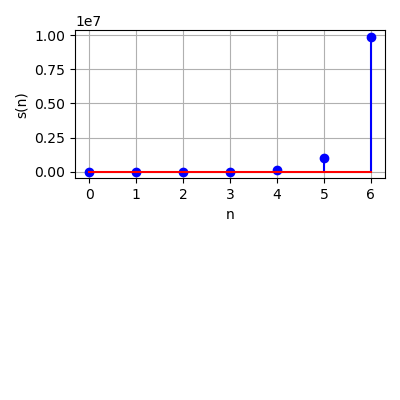
\includegraphics[width=\columnwidth]{figs/plot.png}
    \caption{graph of sum of n terms}
    \label{fig:1}
\end{figure}
 \end{document}
